\section{Results}
\label{sec:Results}

\paragraph{Automatic Evaluation}
Across all architectures, SFT improves Avg by 0.186--0.363 and compilation rate by 19.0--39.3 percentage points. RL further improves EdiTikZ-4B/9B to 0.674/0.726 Avg. EdiTikZ-4B-RL reaches proprietary-level performance, while EdiTikZ-9B-RL achieves the highest overall score (Table~\ref{tab:editikz_main}). Additional results are in Appendix~\ref{subsec:Results}.

\subparagraph{Model Rankings Reverse after SFT}
Qwen3.5-4B/9B initially underperform Qwen3-VL-4B/8B (0.249/0.345 vs.\ 0.314/0.354 Avg), but surpass them after SFT (0.612/0.643 vs.\ 0.538/0.540), showing that base editing performance does not necessarily reflect task-specific adaptation potential.

\subparagraph{Visual Correctness vs.\ Code Similarity}
Unlike prior TikZ-generation RL, where TED improves after RL~\citep{greisinger2026tikzilla,zeng2026davinci}, ours worsens despite consistent gains across rendered metrics. We hypothesize that editing weakens visual--code coupling, as visually equivalent edits may differ at the code level.

\begin{table*}[t]
\centering
\caption{Results on DaEdiTikZ-Bench. \textbf{Bold} is best while \underline{underline} is second-best.}
\label{tab:editikz_main}
\small
\setlength{\tabcolsep}{5pt}
\renewcommand{\arraystretch}{0.95}

\begin{tabular}{lccccc:c:cc}
\toprule

\textbf{Model} &
\textbf{TED}$\downarrow$ &
\textbf{DSim}$\uparrow$ &
\textbf{EA}$\uparrow$ &
\textbf{SP}$\uparrow$ &
\textbf{VQ}$\uparrow$ &
\textbf{Avg}$\uparrow$ &
\textbf{CR}$\uparrow$ &
\textbf{AT}$\downarrow$ \\
\midrule

GPT-5.6-Sol
& 0.764 & 0.796 & 0.735 & 0.775 & 0.823
& \cellcolor{gray!32}0.673
& 88.3\% & 485 \\

GPT-5.5
& 0.765 & 0.829 & \underline{0.744} & 0.790 & \underline{0.849}
& \cellcolor{gray!33}0.689
& 92.2\% & 488 \\

GPT-5.4
& 0.763 & 0.741 & 0.674 & 0.706 & 0.762
& \cellcolor{gray!25}0.624
& 84.6\% & 487 \\

Gemini-3.1-Pro
& 0.716 & 0.795 & \textbf{0.761} & \underline{0.798} & 0.828
& \cellcolor{gray!34}\underline{0.693}
& 86.5\% & \textbf{384} \\

Gemini-3.6-Flash
& 0.740 & 0.665 & 0.654 & 0.677 & 0.698
& \cellcolor{gray!24}0.591
& 72.2\% & \underline{399} \\

Gemini-3.5-Flash
& 0.737 & 0.676 & 0.656 & 0.678 & 0.718
& \cellcolor{gray!24}0.598
& 74.0\% & 427 \\

\midrule

Qwen3.6-27B
& 0.768 & 0.675 & 0.470 & 0.521 & 0.635
& \cellcolor{gray!20}0.507
& 79.0\% & 547 \\

Qwen3.5-27B
& 0.757 & 0.677 & 0.482 & 0.524 & 0.636
& \cellcolor{gray!20}0.512
& 79.0\% & 490 \\

Qwen2.5-VL-7B
& 0.797 & 0.388 & 0.139 & 0.158 & 0.296
& \cellcolor{gray!7}0.237
& 50.6\% & 689 \\

\midrule

Qwen2.5-VL-3B
& 0.810 & 0.329 & 0.062 & 0.062 & 0.213
& \cellcolor{gray!3}0.171
& 45.9\% & 747 \\

EdiTikZ-3B
& 0.707 & 0.700 & 0.309 & 0.332 & 0.525
& \cellcolor{gray!19}0.432
& 82.2\% & 623 \\

\midrule

Qwen3-VL-4B
& 0.788 & 0.494 & 0.232 & 0.245 & 0.386
& \cellcolor{gray!12}0.314
& 61.9\% & 651 \\

EdiTikZ-4B\textsubscript{Qwen3}
& 0.644 & 0.790 & 0.445 & 0.474 & 0.627
& \cellcolor{gray!24}0.538
& 89.3\% & 567 \\

\midrule

Qwen3-VL-8B
& 0.772 & 0.543 & 0.281 & 0.293 & 0.427
& \cellcolor{gray!13}0.354
& 67.2\% & 509 \\

EdiTikZ-8B
& 0.676 & 0.765 & 0.462 & 0.509 & 0.639
& \cellcolor{gray!22}0.540
& 86.2\% & 579 \\

\midrule

Qwen3.5-4B
& 0.806 & 0.411 & 0.146 & 0.188 & 0.304
& \cellcolor{gray!9}0.249
& 51.4\% & 726 \\

EdiTikZ-4B
& \underline{0.629} & 0.813 & 0.552 & 0.609 & 0.714
& \cellcolor{gray!28}0.612
& 90.7\% & 542 \\

EdiTikZ-4B-RL
& 0.642 & \underline{0.871} & 0.633 & 0.706 & 0.803
& \cellcolor{gray!28}0.674
& \underline{95.2\%} & 494 \\

\midrule

Qwen3.5-9B
& 0.781 & 0.523 & 0.241 & 0.311 & 0.430
& \cellcolor{gray!13}0.345
& 64.1\% & 599 \\

EdiTikZ-9B
& \textbf{0.628} & 0.834 & 0.598 & 0.658 & 0.753
& \cellcolor{gray!30}0.643
& 92.0\% & 545 \\

EdiTikZ-9B-RL
& 0.676 & \textbf{0.893} & 0.734 & \textbf{0.815} & \textbf{0.865}
& \cellcolor{gray!35}\textbf{0.726}
& \textbf{96.8\%} & 488 \\

\bottomrule
\end{tabular}
\end{table*}

\paragraph{Human Evaluation}
We conduct a human evaluation with 9 qualified annotators, who rate predictions from eight models on EA, SP, and VQ using a 1--7 Likert scale (Figure~\ref{fig:human_evaluation}). Each annotator evaluates 20 randomized figure groups with 10\% overlap, yielding 4,320 ratings. Quadratic-weighted agreement is high ($\kappa_{\mathrm{EA}}=0.801$, $\kappa_{\mathrm{SP}}=0.786$, $\kappa_{\mathrm{VQ}}=0.832$).

\subparagraph{Human Evaluation Confirms Post-Training Gains}
SFT raises the combined score of Qwen3.5-4B/9B from 6.40/8.78 to 14.71/15.18, with RL further improving it to 16.14/17.43, with gains across all three criteria. EdiTikZ-9B-RL nearly matches Gemini-3.1-Pro (17.43 vs.\ 17.72) and performs above GPT-5.6-Sol (16.75). SFT narrows the 4B--9B gap from 2.38 to 0.47 points, whereas RL widens it to 1.29 points.

\subparagraph{Automatic Metrics Align with Humans}
Our aggregate metric correlates strongly with combined human judgments ($\rho=0.823$). While TED correlates poorly ($\rho=0.374$), DSim and the criterion-specific EA, SP, and VQ metrics each reach $\rho\approx0.77$. $\mathcal{R}_{\mathrm{SSim}}$ correlates more strongly with human SP/VQ, whereas adding $\mathcal{R}_{\mathrm{IF}}$ improves EA correlation by 0.045 and raises overall correlation from 0.812 to 0.827, showing the intended complementarity.

\begin{figure}[h]
  \centering
  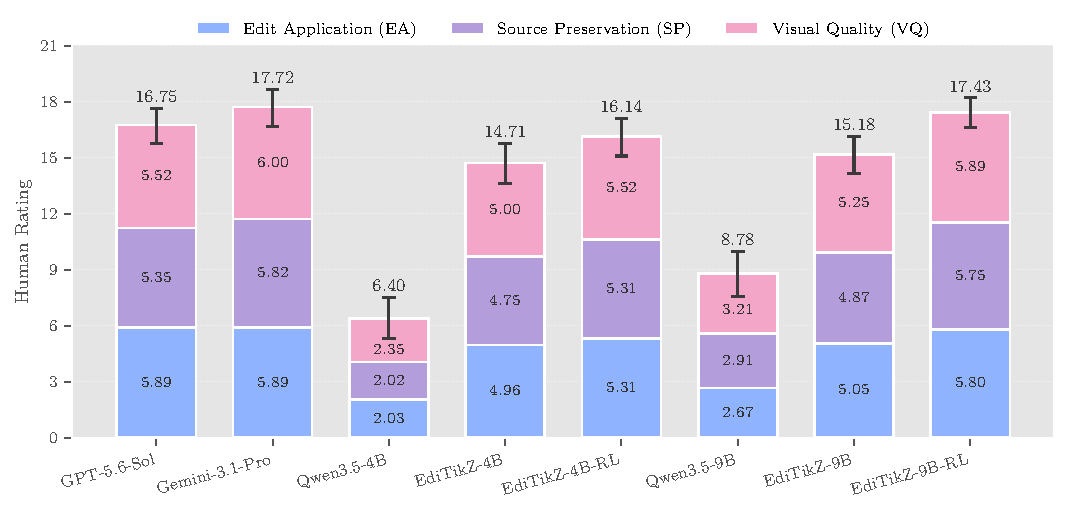
\includegraphics[width=0.85\textwidth]{structure/figures/human_evaluation.pdf}
  \caption{Likert-scale (1-7) across three evaluation criteria (EA, SP, and VQ) with 95\% confidence intervals for eight VLMs (4 baseline, 4 fine-tuned).}
  \label{fig:human_evaluation}
\end{figure}

\paragraph{Ablations: Data Mixtures}
Table~\ref{tab:editikz_ablation_data_mixture_new} compares reconstruction and editing mixtures on two VLMs. Joint training performs best for 3B (0.432 Avg vs.\ 0.392 editing-only) and matches sequential training for 8B (0.539/0.540), with both exceeding editing-only (0.531). Thus, reconstruction consistently improves editing, while joint training additionally retains both capabilities.

\paragraph{Ablations: Rewards and GDPO}
Table~\ref{tab:editikz_ablation_rl_new} ablates our rewards and optimization algorithm. $\mathcal{R}_{\mathrm{IF}}$ outperforms $\mathcal{R}_{\mathrm{SSim}}$, by +0.031 EA. Combining both with GRPO adds +0.009 Avg, while GDPO increases this gain to +0.038, supporting independent normalization of the complementary rewards.

\begin{table*}[t]
\centering
\tiny
\setlength{\tabcolsep}{1.2pt}
\renewcommand{\arraystretch}{0.92}

\begin{minipage}[t]{0.53\textwidth}
\centering
\caption{Ablation on DaEdiTikZ-Bench for data-mixing strategies on two VLMs.}
\label{tab:editikz_ablation_data_mixture_new}

\begin{tabular}{clccccc:c:cc}
\toprule
\textbf{VLM} &
\textbf{Variant} &
\textbf{TED}$\downarrow$ &
\textbf{DSim}$\uparrow$ &
\textbf{EA}$\uparrow$ &
\textbf{SP}$\uparrow$ &
\textbf{VQ}$\uparrow$ &
\textbf{Avg}$\uparrow$ &
\textbf{CR}$\uparrow$ &
\textbf{AT}$\downarrow$ \\
\midrule

\multirow{5}{*}{%
\rotatebox{90}{%
\fontsize{4.5}{5.1}\selectfont
\textbf{Qwen2.5-VL-3B}%
}%
}
& Base
& 0.810 & 0.329 & 0.062 & 0.062 & 0.213
& \cellcolor{gray!3}0.171
& 45.9\% & 747 \\

& Only Recon
& 0.751 & 0.615 & 0.016 & 0.277 & 0.426
& \cellcolor{gray!16}0.317
& 68.4\% & 800 \\

& Only Edit
& 0.741 & 0.626 & \underline{0.296} & \underline{0.309}
& 0.472
& \cellcolor{gray!22}0.392
& 73.9\% & 723 \\

& Recon$\rightarrow$Edit
& \underline{0.720} & \underline{0.647} & 0.272 & 0.297
& \underline{0.480}
& \cellcolor{gray!22}\underline{0.395}
& \underline{76.2\%} & \underline{686} \\

& Recon+Edit
& \textbf{0.707} & \textbf{0.700} & \textbf{0.309} & \textbf{0.332}
& \textbf{0.525}
& \cellcolor{gray!26}\textbf{0.432}
& \textbf{82.2\%} & \textbf{623} \\

\midrule

\multirow{5}{*}{%
\rotatebox{90}{%
\fontsize{4.5}{5.1}\selectfont
\textbf{Qwen3-VL-8B}%
}%
}
& Base
& 0.772 & 0.543 & 0.281 & 0.293 & 0.427
& \cellcolor{gray!19}0.354
& 67.2\% & \textbf{509} \\

& Only Recon
& 0.709 & 0.737 & 0.157 & 0.495 & 0.592
& \cellcolor{gray!28}0.454
& 85.1\% & 646 \\

& Only Edit
& 0.713 & 0.785 & 0.451 & 0.493 & 0.638
& \cellcolor{gray!34}0.531
& \textbf{90.6\%} & \underline{557} \\

& Recon$\rightarrow$Edit
& \underline{0.685} & \textbf{0.769} & \underline{0.459} & \textbf{0.512}
& \textbf{0.640}
& \cellcolor{gray!35}\underline{0.539}
& \underline{87.1\%} & 593 \\

& Recon+Edit
& \textbf{0.676} & \underline{0.765} & \textbf{0.462} & \underline{0.509}
& \underline{0.639}
& \cellcolor{gray!35}\textbf{0.540}
& 86.2\% & 579 \\

\bottomrule
\end{tabular}
\end{minipage}
\hfill
\begin{minipage}[t]{0.45\textwidth}
\centering
\caption{Ablation on DaEdiTikZ-Bench for reward functions and algorithms using EdiTikZ-9B.}
\label{tab:editikz_ablation_rl_new}

\setlength{\tabcolsep}{1.2pt}
\begin{tabular}{lccccc:c:cc}
\toprule
\textbf{Variant} &
\textbf{TED}$\downarrow$ &
\textbf{DSim}$\uparrow$ &
\textbf{EA}$\uparrow$ &
\textbf{SP}$\uparrow$ &
\textbf{VQ}$\uparrow$ &
\textbf{Avg}$\uparrow$ &
\textbf{CR}$\uparrow$ &
\textbf{AT}$\downarrow$ \\
\midrule

Post-SFT
& \textbf{0.628} & 0.834 & 0.598 & 0.658
& 0.753
& \cellcolor{gray!3}0.643
& 92.0\% & 545 \\

\midrule

$\mathcal{R}_{\mathrm{SSim}}$
& 0.667 & 0.872 & 0.633 & 0.706
& 0.805
& \cellcolor{gray!13}0.670
& 96.1\% & 489 \\

$\mathcal{R}_{\mathrm{IF}}$
& 0.671 & 0.866 & 0.664 & 0.721
& 0.814
& \cellcolor{gray!17}0.679
& 95.2\% & \underline{488} \\

Both (w. GRPO)
& \underline{0.662} & \underline{0.879}
& \underline{0.671} & \underline{0.728}
& \underline{0.822}
& \cellcolor{gray!20}\underline{0.688}
& \underline{96.4\%} & \textbf{476} \\

Both (w. GDPO)
& 0.676 & \textbf{0.893}
& \textbf{0.734} & \textbf{0.815}
& \textbf{0.865}
& \cellcolor{gray!35}\textbf{0.726}
& \textbf{96.8\%} & \underline{488} \\

\bottomrule
\end{tabular}
\end{minipage}

\end{table*}

\paragraph{Generalization under Severe Distribution Shift}
We stress-test EdiTikZ on SPIQA~\cite{NEURIPS2024_SPIQA} and CharXiv~\cite{NEURIPS2024_CharXiv}, which contain complex architectural diagrams, multi-panel plots, tables, schematics, and charts across diverse scientific domains, produced with tools such as Matplotlib, MATLAB, DrawIO, ggplot, and Plotly rather than TikZ. We sample 300 SPIQA and 600 CharXiv figures and manually remove those requiring external data, leaving 190 and 497 instances, respectively. Since neither dataset provides editing pairs, we use GPT-5.6-Sol to generate synthetic edit instructions. We then evaluate model predictions reference-free using EA, SP, VQ, CR, and AT. OOD generations require $3$--$5\times$ more tokens than DaEdiTikZ-Bench and frequently exceed the 2K-token completion limit used during post-training. We stratify examples by mean generation length across all four models (Figure~\ref{fig:ood_evaluation}), ensuring identical examples within each bin.

\subparagraph{RL Gains Increase with Difficulty}
For short generations ($<$1K), SFT provides most of the gain over Qwen3.5-9B. With increasing length, SFT gains diminish while the additional benefit from RL grows, dominating from 1.5--4K tokens. RL also maintains $>$80\% compilation through 3--4K, consistently exceeding GPT-5.6-Sol, whereas SFT compilation degrades steadily.

\subparagraph{Competitive within the Training Horizon}
Within the trained $\leq$2K regime, EdiTikZ-9B-RL remains close to GPT-5.6-Sol, with $<$0.1 Avg difference across all bins. Beyond 2K, EdiTikZ degrades faster and the gap widens, although SFT and RL gains persist throughout the 2--8K regime.

\begin{figure}[h]
  \centering
  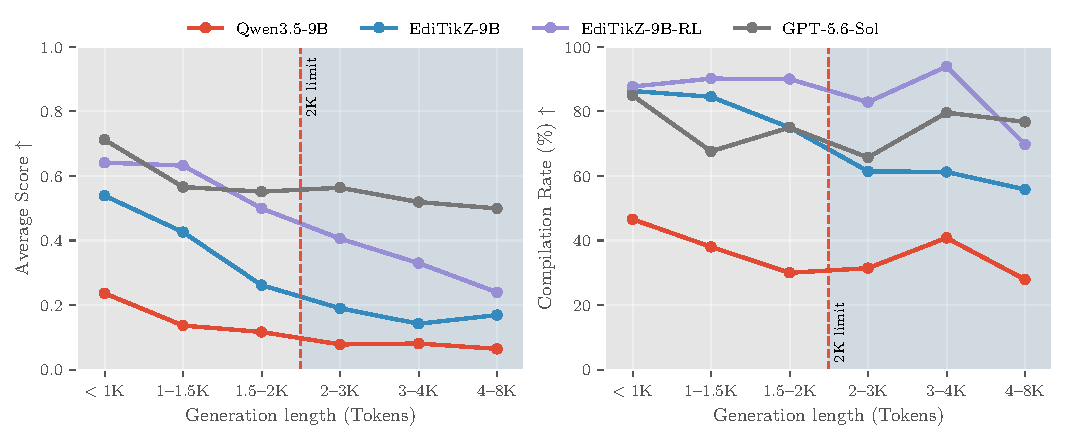
\includegraphics[width=0.75\textwidth]{structure/figures/ood_length_generalization_main.pdf}
  \caption{OOD performance on SPIQA and CharXiv combined by generation length. Average score is $(\mathrm{EA}+\mathrm{SP}+\mathrm{VQ})/3$. The red dashed line marks the 2K-token post-training limit.}
  \label{fig:ood_evaluation}
\end{figure}